\begin{figure}\centering
	\subfloat[]{%
		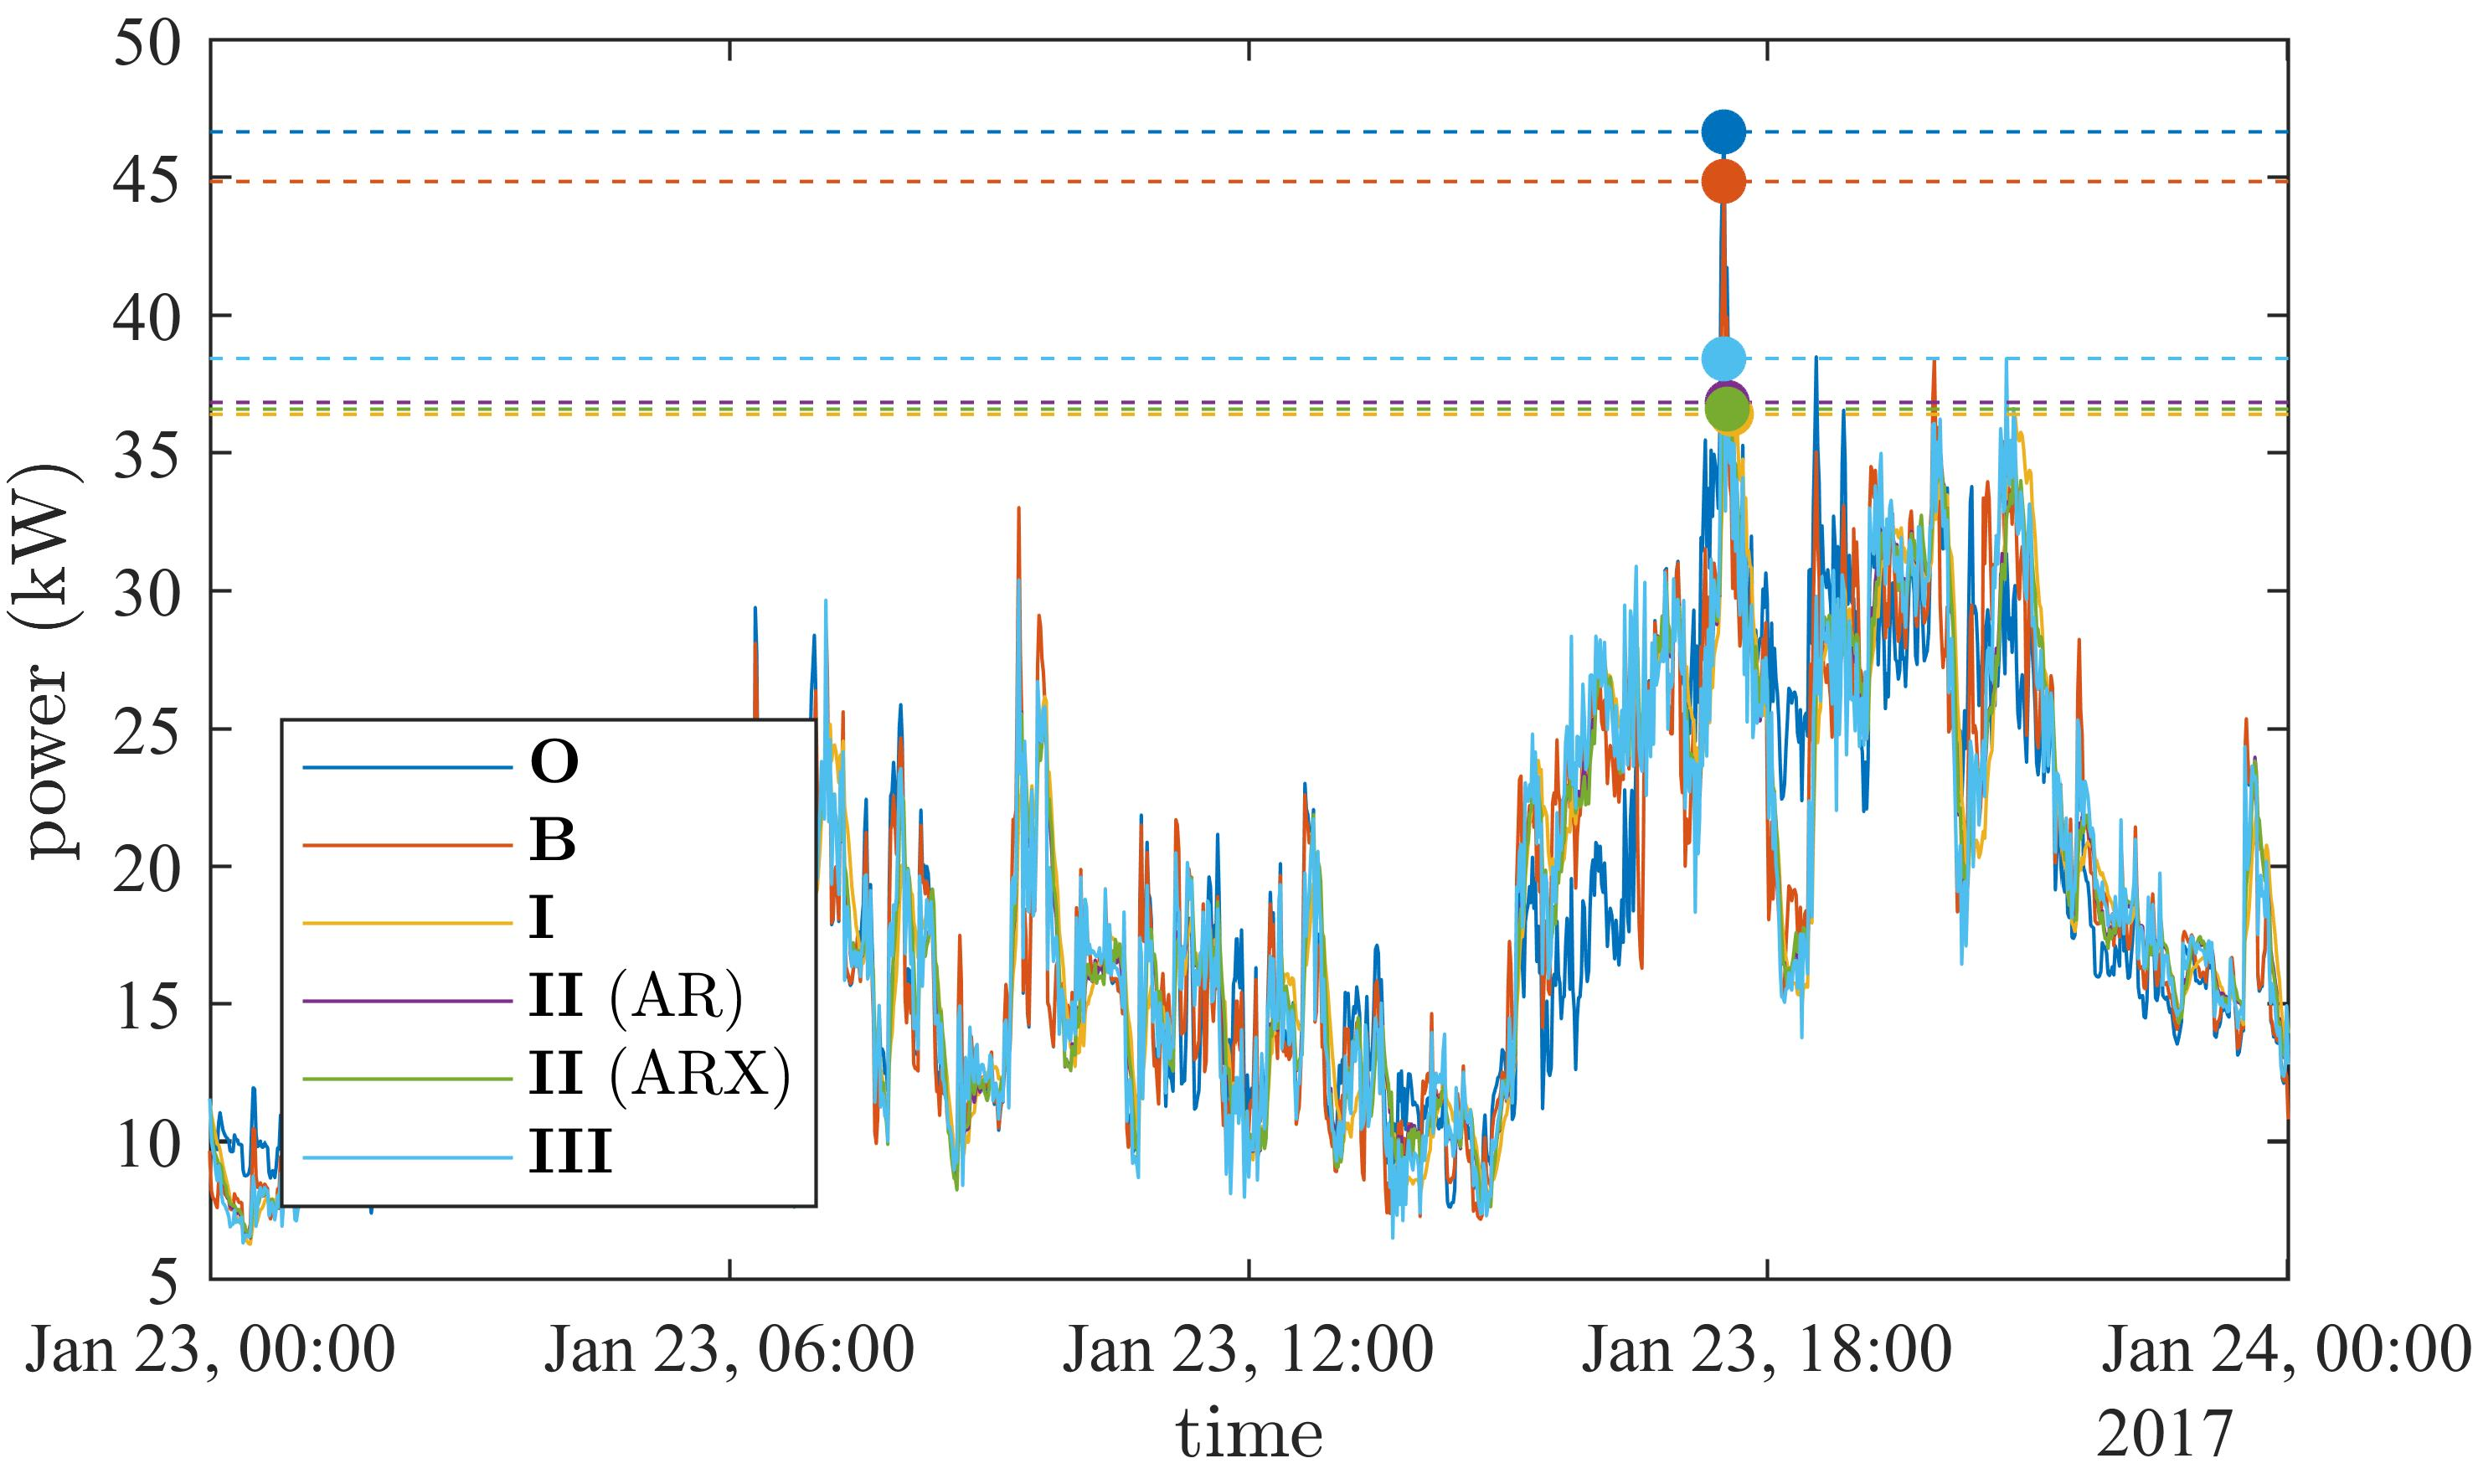
\includegraphics{_chapter2/fig/day-peak-1}
		\label{ch2:subfig:day-peak-total}
	}\\
	\subfloat[]{%
		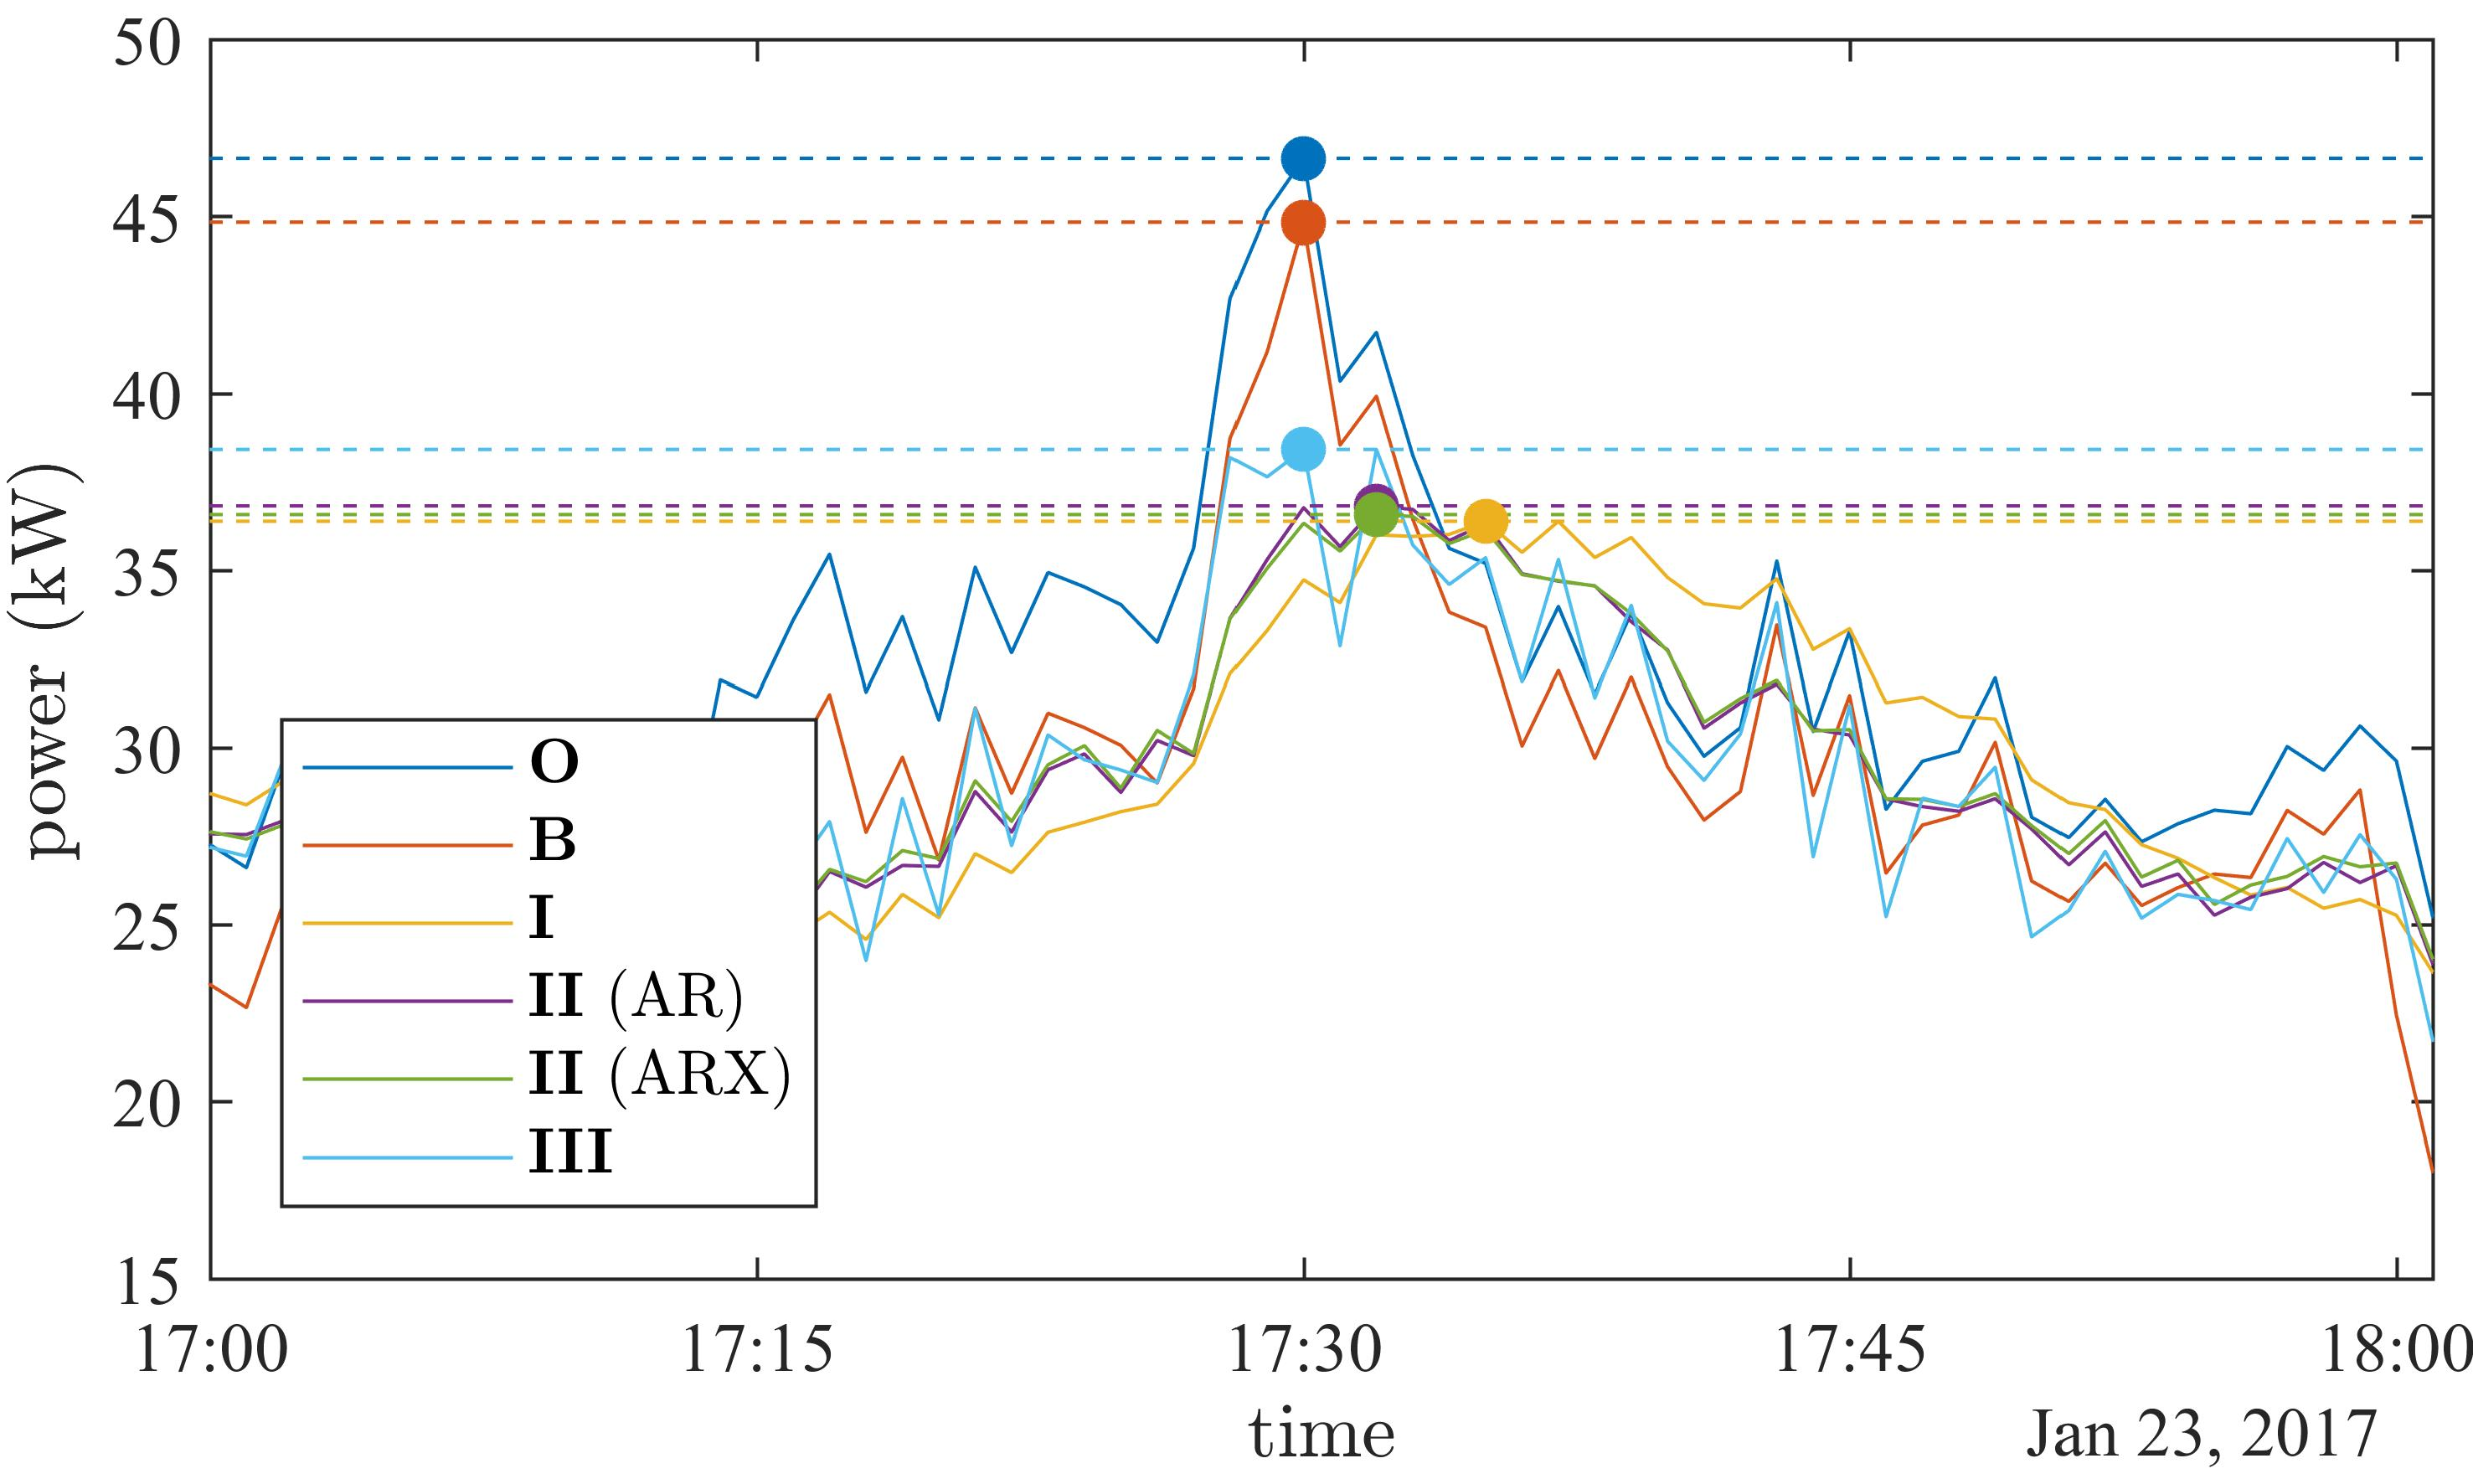
\includegraphics{_chapter2/fig/day-peak-1-zoom}
		\label{ch2:subfig:day-peak-zoomed}
	}
%	\subfloat[]{%
%		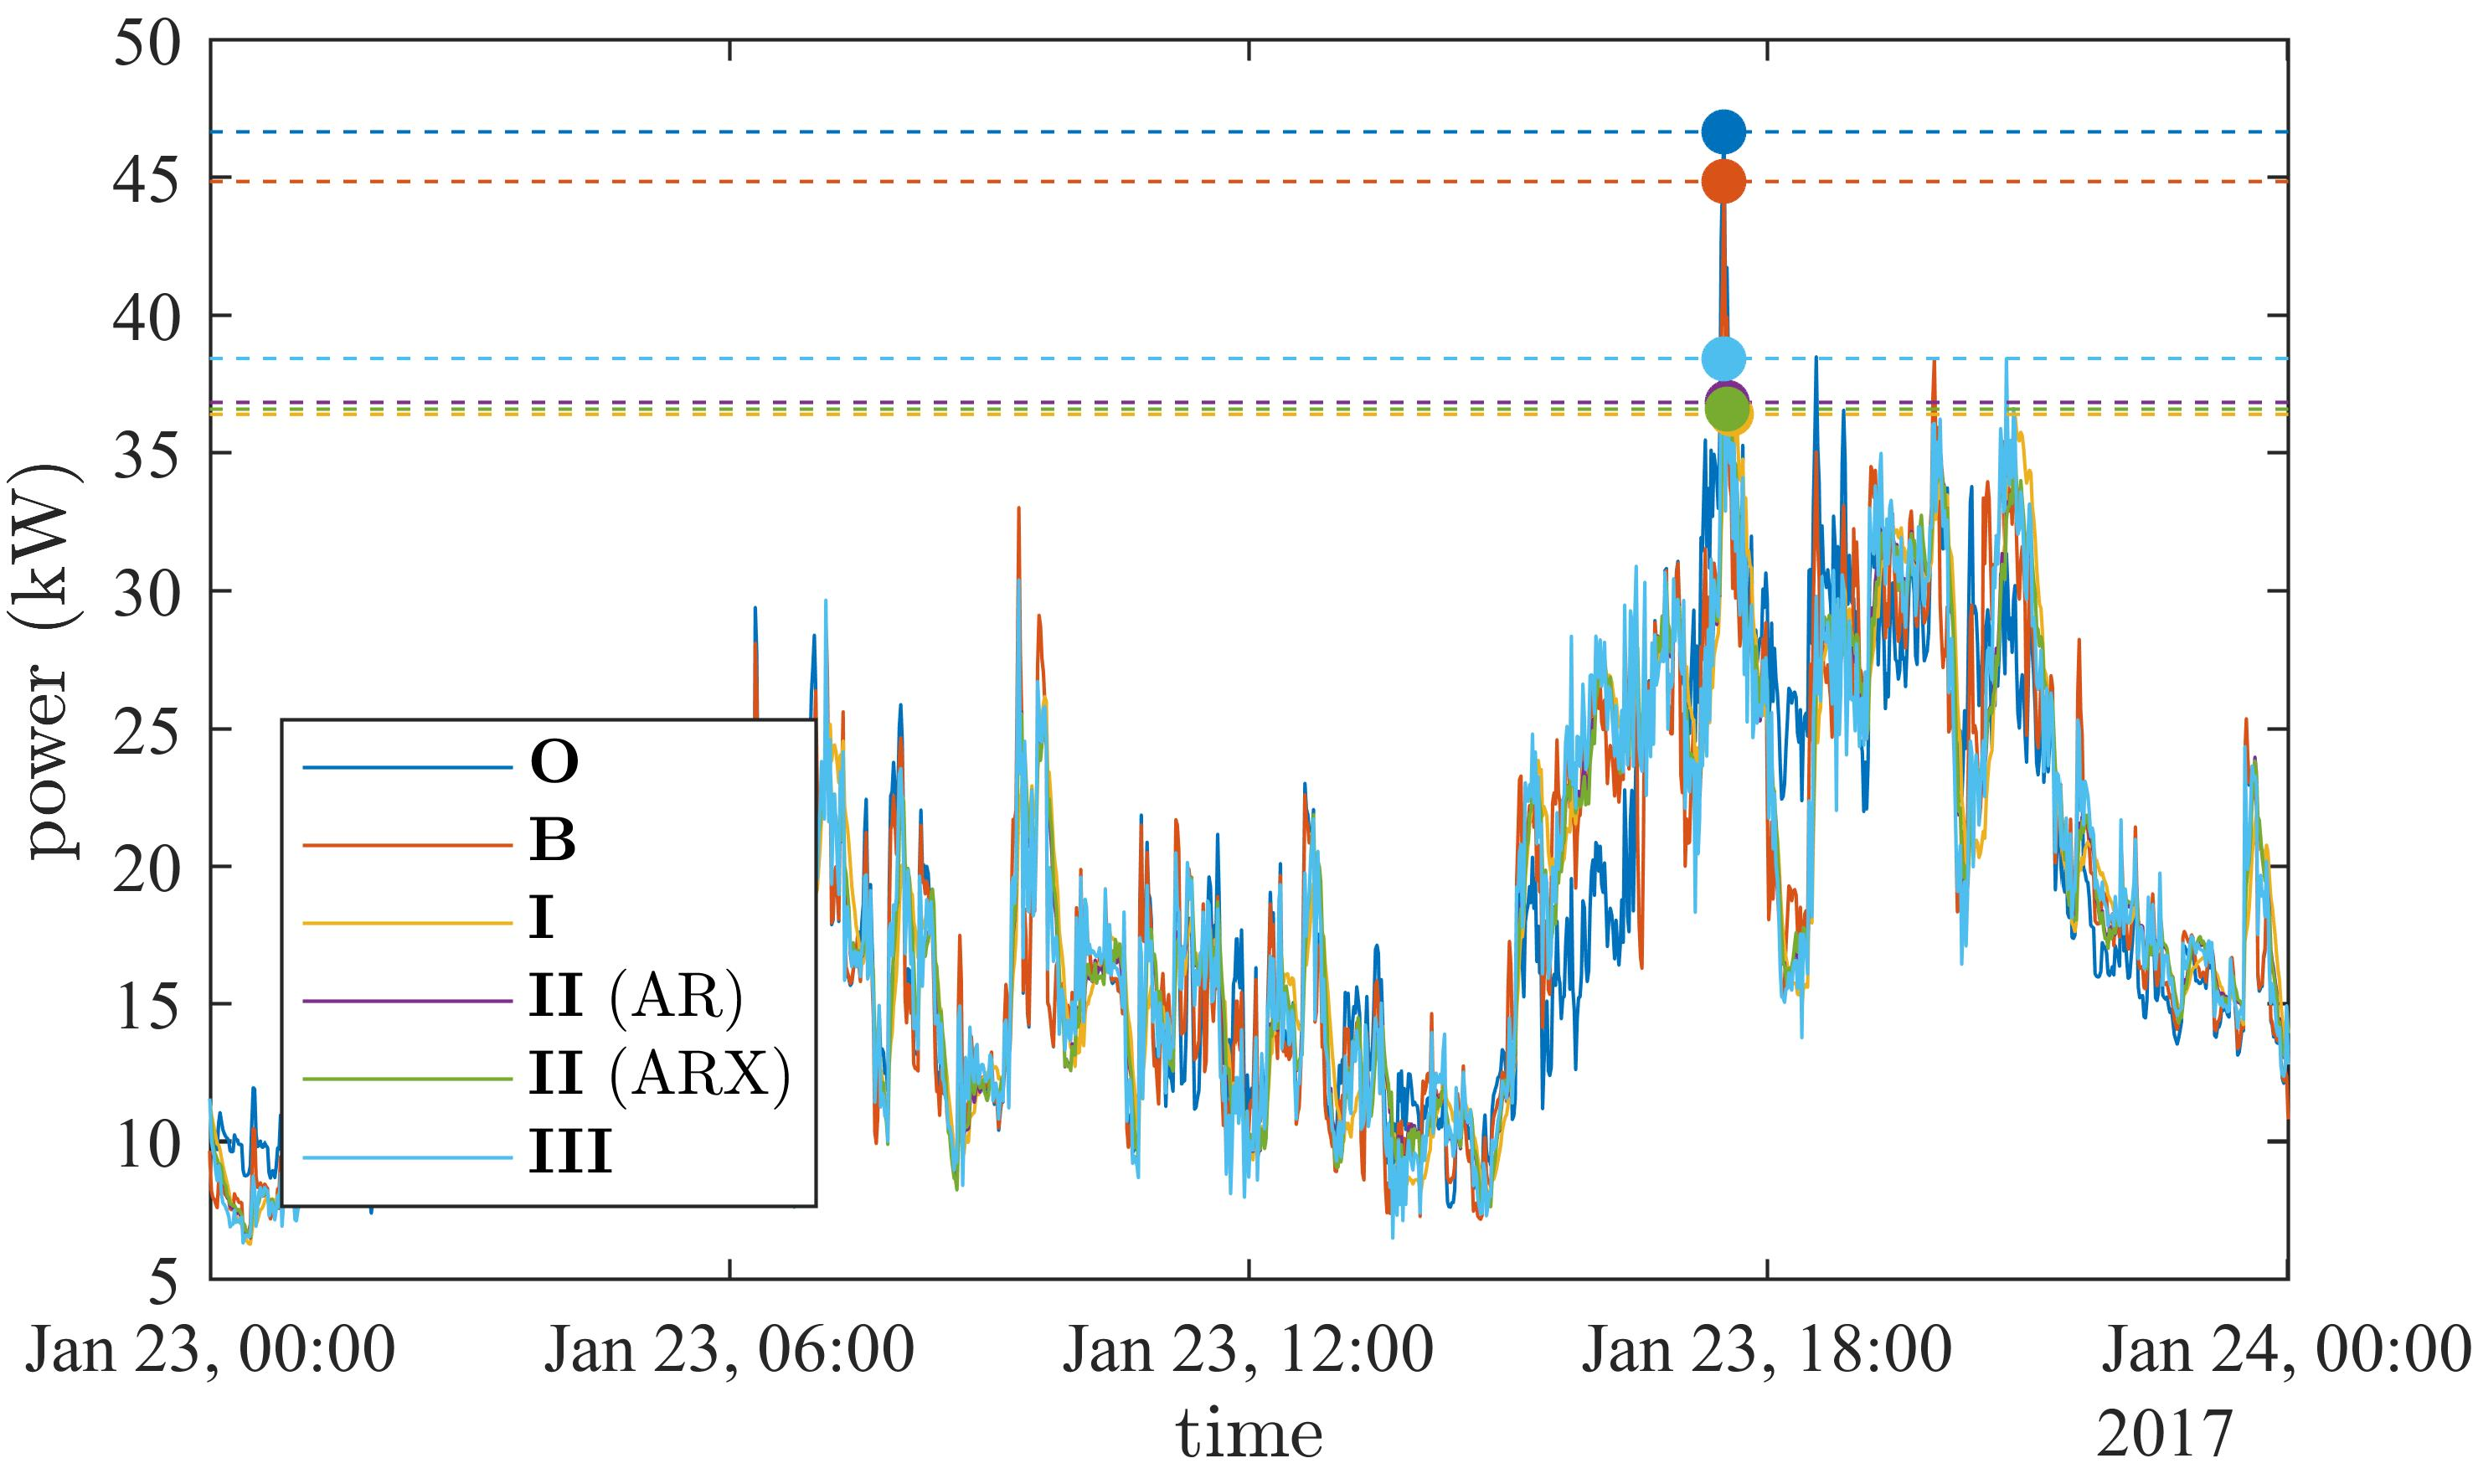
\includegraphics{_chapter2/fig/day-peak-1}
%		\label{ch2:subfig:day-peak-1}
%	}
%	\vspace{0mm}
%	\subfloat[]{%
%		\includegraphics{_chapter2/fig/day-peak-2}
%		\label{ch2:subfig:day-peak-2}
%	}
	\caption{Time series performance over a single day when using realistic load forecasts: (\ref{ch2:subfig:day-peak-total}) total day; (\ref{ch2:subfig:day-peak-zoomed}) zoomed in on critical period}
	\label{ch2:fig:day-peak}
\end{figure}